%%%%%%%%%%%%%%%%%%%%%%%%%%%%%%%%%%%%%%%%%%%%%%%%%%%%%%%%%%%%%%%%%%%%%%%%
\chapter{Results}
\label{sec:results}
%%%%%%%%%%%%%%%%%%%%%%%%%%%%%%%%%%%%%%%%%%%%%%%%%%%%%%%%%%%%%%%%%%%%%%%%

\section{Algorithm-level compatibility}

The most important part of this work was to port the Lyra2 PHS to Java in such a way that the program would produce exactly the same hashes as the original C implementation. Of course, formal verification would be the ideal way of proving the two implementations to be identical. However, this is definitely even more work than porting from one language into the other. Therefore, the following two-step approach is used instead: there are several manual tests followed by a larger collection of randomly generated tests.

\subsection{Configuration choice}
By design Lyra2 provides a large number of possible configurations and modes of operation. This section will provide rationale for choosing particular values for the configuration parameters. The summary can be found in the following table \ref{table:configuration-summary}.

There are three sponges that could be tested: Blake2b, BlaMka and half-round BlaMka. Just the first two are in the manual testing shortlist because half-round BlaMka is similar to BlaMka. The sponge block size can be either 8, 10 or 12, so the extreme values make it into the shortlist. The columns of the memory matrix can be any positive number, so the values of 256 and 512 are chosen, primarily because 256 is used in the original paper. Finally, time and memory cost are fixed at an arbitrary value of 100 and the output length is 10 for representation purposes.

\begin{table}
\begin{center}
\begin{tabular}{l r}
Parameter & Value \\ \hline
Sponge & Blake2b, BlaMka \\
Sponge blocks & 8, 12 \\
Columns in the memory matrix & 256, 512 \\
Time cost (number of iterations) & 100 \\
Memory cost (number of rows in the memory matrix) & 100 \\
Output length (bytes) & 10 \\
\end{tabular}
\end{center}
\caption{Summary of parameter values for tested configurations}
\label{table:configuration-summary}
\end{table}

\subsection{Manual testing}

Below is a log of manual tests. New line delimits different lyra2 configurations. The first line of each group represents the particular configuration group: \verb|--outlen| is the output length, \verb|--tcost| is the time cost, \verb|--mcost| is memory cost. The second and the forth line in each group is the password and salt pair, and the third and fifth lines are the resulting hash values.

\tiny
\begin{verbatim}
$ lyra2 --sponge blake2b --blocks 8 --columns 256 --outlen 10 --tcost 100 --mcost 100
> "password" "salt"
> 19 FD 3B 50 9A 03 0C DF 95 DA
> "The quick brown fox jumped over the lazy dog" "0123456789"
> 04 A0 BF 30 D1 E5 A5 05 53 E9

$ lyra2 --sponge blake2b --blocks 8 --columns 512 --outlen 10 --tcost 100 --mcost 100
> "password" "salt"
> 73 39 79 B6 C1 3C C1 F3 D7 17
> "The quick brown fox jumped over the lazy dog" "0123456789"
> A1 B0 18 F6 B6 79 5F E0 2A A4

$ lyra2 --sponge blake2b --blocks 12 --columns 256 --outlen 10 --tcost 100 --mcost 100
> "password" "salt"
> 9C 52 2A B9 18 30 F9 E7 09 55
> "The quick brown fox jumped over the lazy dog" "0123456789"
> 7D B2 9D C8 31 B4 E9 0E 10 22

$ lyra2 --sponge blake2b --blocks 12 --columns 512 --outlen 10 --tcost 100 --mcost 100
> "password" "salt"
> AC F2 B6 50 2D BC F0 62 DD 29
> "The quick brown fox jumped over the lazy dog" "0123456789"
> 4F 1B 03 6B C9 A2 09 C4 BC DA

$ lyra2 --sponge blamka --blocks 8 --columns 256 --outlen 10 --tcost 100 --mcost 100
> "password" "salt"
> 53 32 F3 D7 C4 9C 46 38 3C 1B
> "The quick brown fox jumped over the lazy dog" "0123456789"
> E7 6E 4B A0 81 B8 3C CF D6 64

$ lyra2 --sponge blamka --blocks 8 --columns 512 --outlen 10 --tcost 100 --mcost 100
> "password" "salt"
> D9 F9 F5 65 0D 05 88 D0 DF F6
> "The quick brown fox jumped over the lazy dog" "0123456789"
> 3A 3D 40 00 3E 33 44 45 B3 DD

$ lyra2 --sponge blamka --blocks 12 --columns 256 --outlen 10 --tcost 100 --mcost 100
> "password" "salt"
> C1 BC 48 80 99 1C E7 E6 52 18
> "The quick brown fox jumped over the lazy dog" "0123456789"
> 2E 4E 56 C7 5B 3D B7 F9 E0 30

$ lyra2 --sponge blamka --blocks 12 --columns 512 --outlen 10 --tcost 100 --mcost 100
> "password" "salt"
> 82 AF EB 03 5B E7 12 11 BE 63
> "The quick brown fox jumped over the lazy dog" "0123456789"
> F7 A8 56 D5 81 16 AA E5 C7 4D
\end{verbatim}
\normalsize

\subsection{Automated testing}

For automated testing a separate test harness was developed for the original Lyra2 implementation. It is located in the \verb|Lyra2/tests| directory on the \verb|harness| branch of the \href{https://github.com/all3fox/Lyra/tree/harness}{Lyra2 fork}. There is a \href{https://github.com/leocalm/Lyra/pull/7}{corresponding pull request} to the original Lyra2 repository. In short, the \texttt{./tests/harness.py compile} script will compile several Lyra2 configurations at once. The exact configurations can be adjusted in \verb|tests/harness.yml|. After the compilation step, the \texttt{./tests/harness.py compute} will compute a number of hash values for you (the exact details for runtime parameters such as \verb|password|, \verb|salt| and so on can again be configured via \verb|harness.yml|). Finally, the \verb|tests/take.py| script will choose \verb|N| random hash values for you and prepare them to be used as unit-testing data for the Java implementation.

There are not less than 600 randomly chosen unit-tests which are currently included into a continuous integration cycle on the Travis CI service through the Maven build system and the JUnit testing library. Testing status can be \href{https://travis-ci.org/all3fox/lyra2-java}{checked here}.

\section{Performance comparison}

To perform comparison of the original C implementation and its ported Java version, a separate project was created and is hosted in \href{https://github.com/all3fox/lyra2-compare}{a public GitHub repository}. At the core of this project lies the open-source \href{https://jupyter.org/}{Jupyter Notebook} which simplifies reproduction of comparison results.

The following producer-consumer strategy is employed. The producer is the \texttt{./src/compare.ipynb} script which is responsible for compiling both C and Java implementations as well as dispatching computation tasks. The results are then collected into the \texttt{measurements.db} SQLite database (which also serves as a cache layer). The consumer is the \texttt{./src/plot.ipynb} script which reads the data from the SQLite database and plots the figures shown below.

Conceptually, Lyra2 provides two main adjustable parameters: time and memory cost. This is why this performance comparison includes sections where one of these parameters is fixed and the other is changed. This is done for several Lyra2 configurations and their running time as well as memory consumption is compared. For the exact comparison steps you could consult \href{https://github.com/all3fox/lyra2-compare/blob/master/src/compare.ipynb}{the script} but here is a quick summary:

\begin{itemize}
\item Separate configurations are run in parallel, creating one process per configuration.
\item Running time is measured as the time between the creation of the process and its termination.
\item Memory consumption of the created process is measured externally and the peak value is recorded.
\end{itemize}

There is also a section where both time and memory costs are changed at the same time. This produces 3-dimensional plots. Direct comparison of such plots is difficult but they still provide a good feel for how the running time and memory consumption are changing.

\subsection{Fixed time cost}

There are two figures that show how running time and consumed memory depend on memory cost when the time cost is fixed. Figure \ref{figure:mcost_256} shows a 256-column and figure \ref{figure:mcost_2048} shows a 2048-column configuration of Lyra2. Both these figures clearly show that the original C implementation works faster and consumes less memory than its Java counterpart. A nice property is that both the running time and memory consumption are changing roughly linearly as the memory cost parameter is changed. This is consistent with the fact that the memory cost parameter corresponds to the number of rows of the in-memory matrix.

\begin{figure}
    \centering
    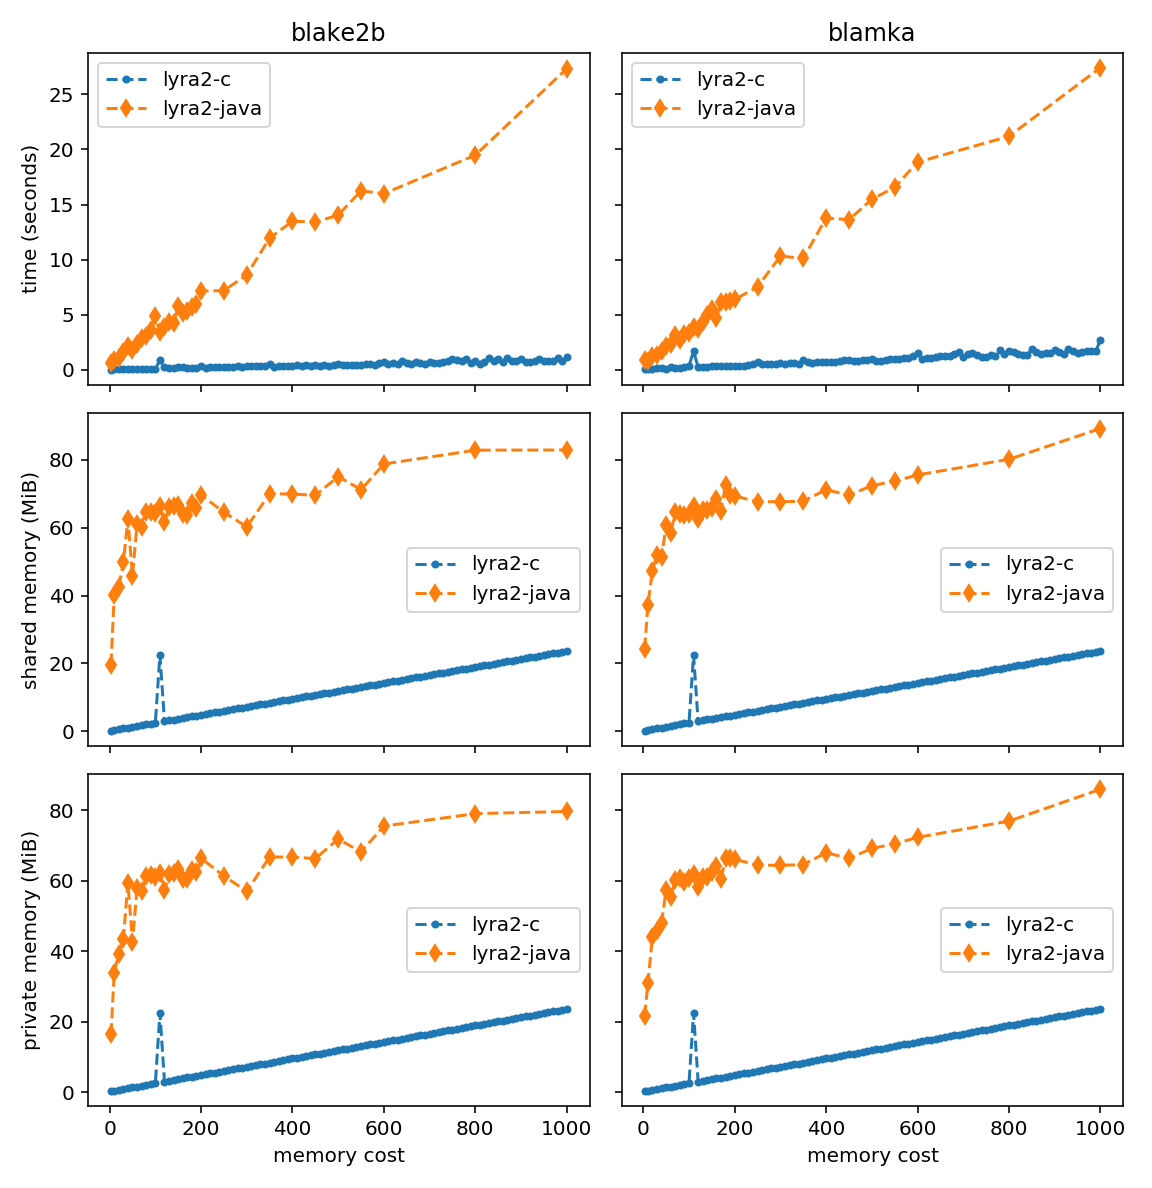
\includegraphics[width=\linewidth]{figures/mcost_256}
    \caption{Original \texttt{lyra2-c} compared to \texttt{lyra2-java}: 256 columns, fixed time cost of 10}
    \label{figure:mcost_256}
\end{figure}

\begin{figure}
    \centering
    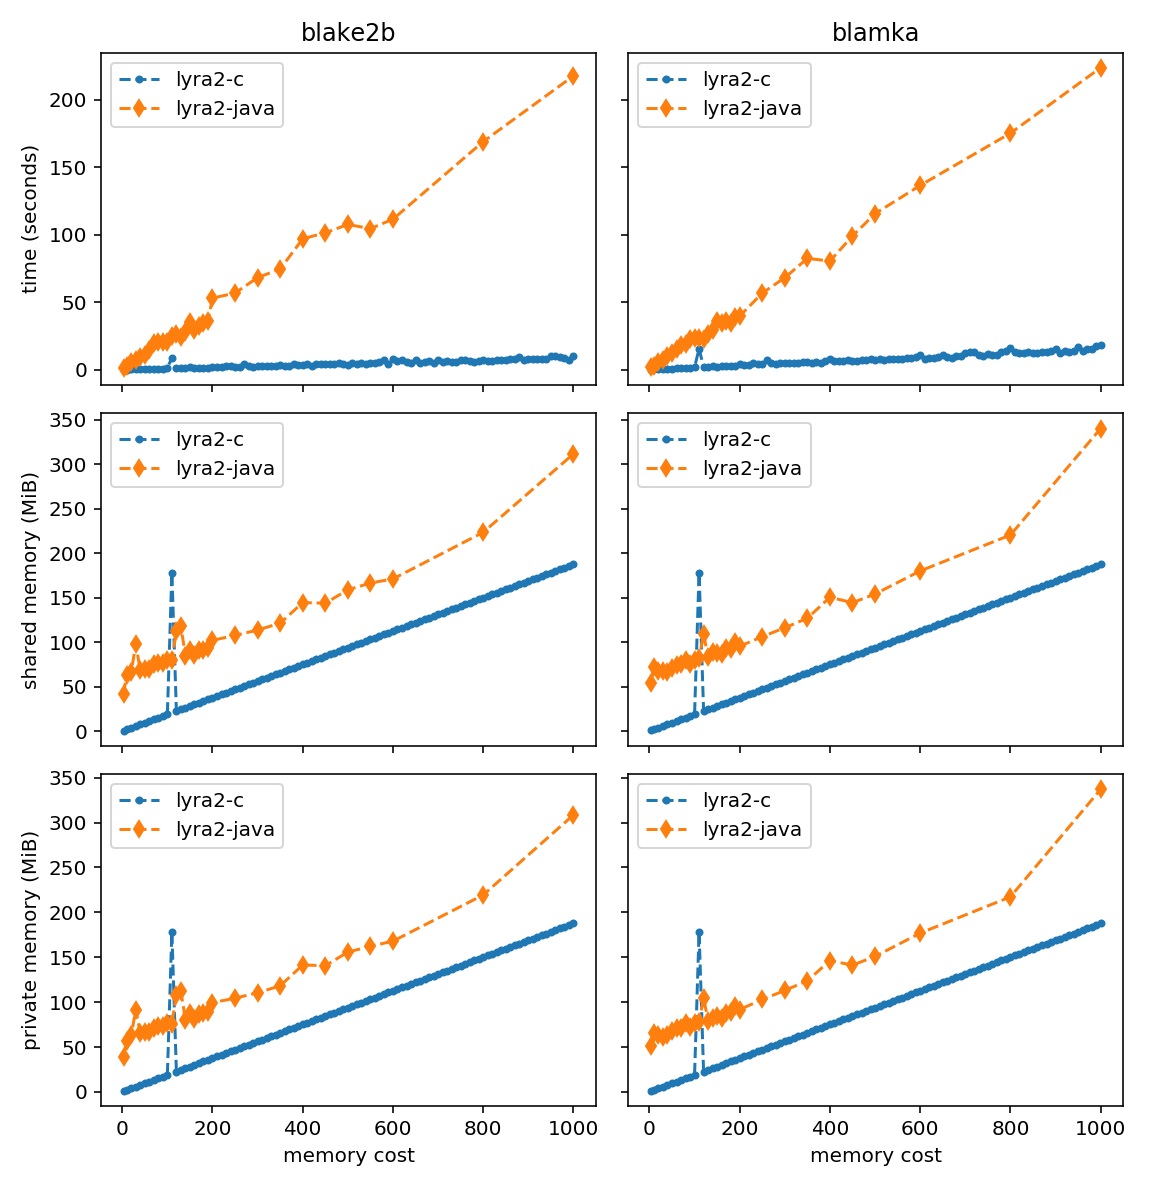
\includegraphics[width=\linewidth]{figures/mcost_2048}
    \caption{Original \texttt{lyra2-c} compared to \texttt{lyra2-java}: 2048 columns, fixed time cost of 10}
    \label{figure:mcost_2048}
\end{figure}

\subsection{Fixed memory cost}

There are two figures that show how running time and consumed memory depend on time cost when the memory cost is fixed. Figure \ref{figure:tcost_256} shows a 256-column and figure \ref{figure:tcost_2048} shows a 2048-column configuration of Lyra2. Both these figures clearly show that the original C implementation works faster and consumes less memory than its Java counterpart.
The running time changes roughly linearly as the time cost parameter is changed which is consistent with the fact that time cost corresponds to the number of iterations done by Lyra2. Memory consumption stays roughly the same which is also consistent with the fact that the largest memory consumer is the in-memory matrix. This matrix has the same size for all of the configurations.

\begin{figure}
    \centering
    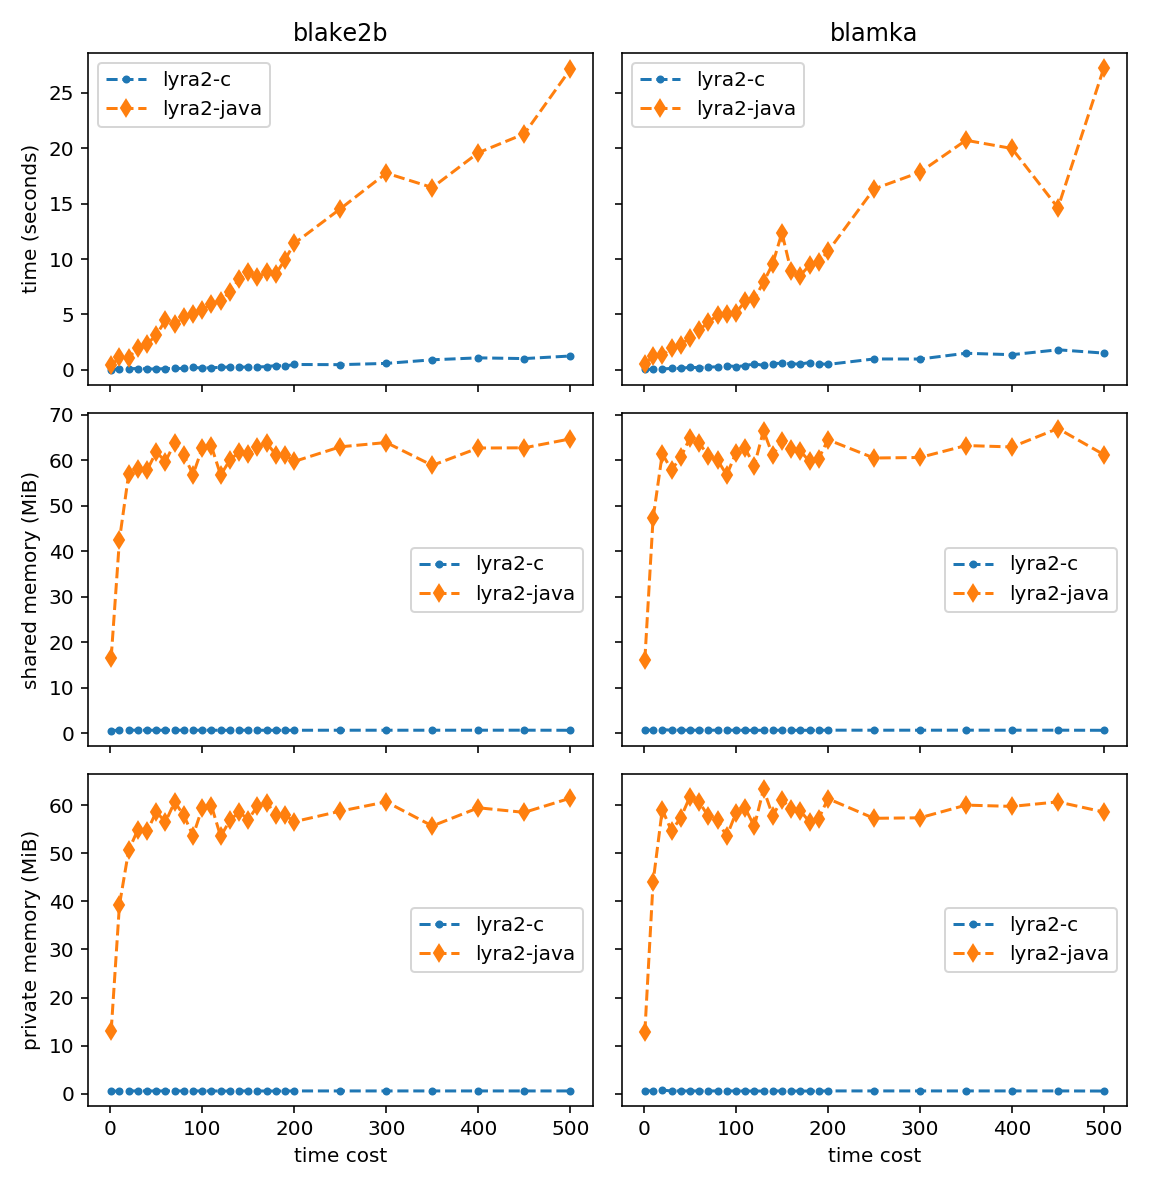
\includegraphics[width=\linewidth]{figures/tcost_256}
    \caption{Original \texttt{lyra2-c} compared to \texttt{lyra2-java}: 256 columns, fixed memory cost of 20}
    \label{figure:tcost_256}
\end{figure}

\begin{figure}
    \centering
    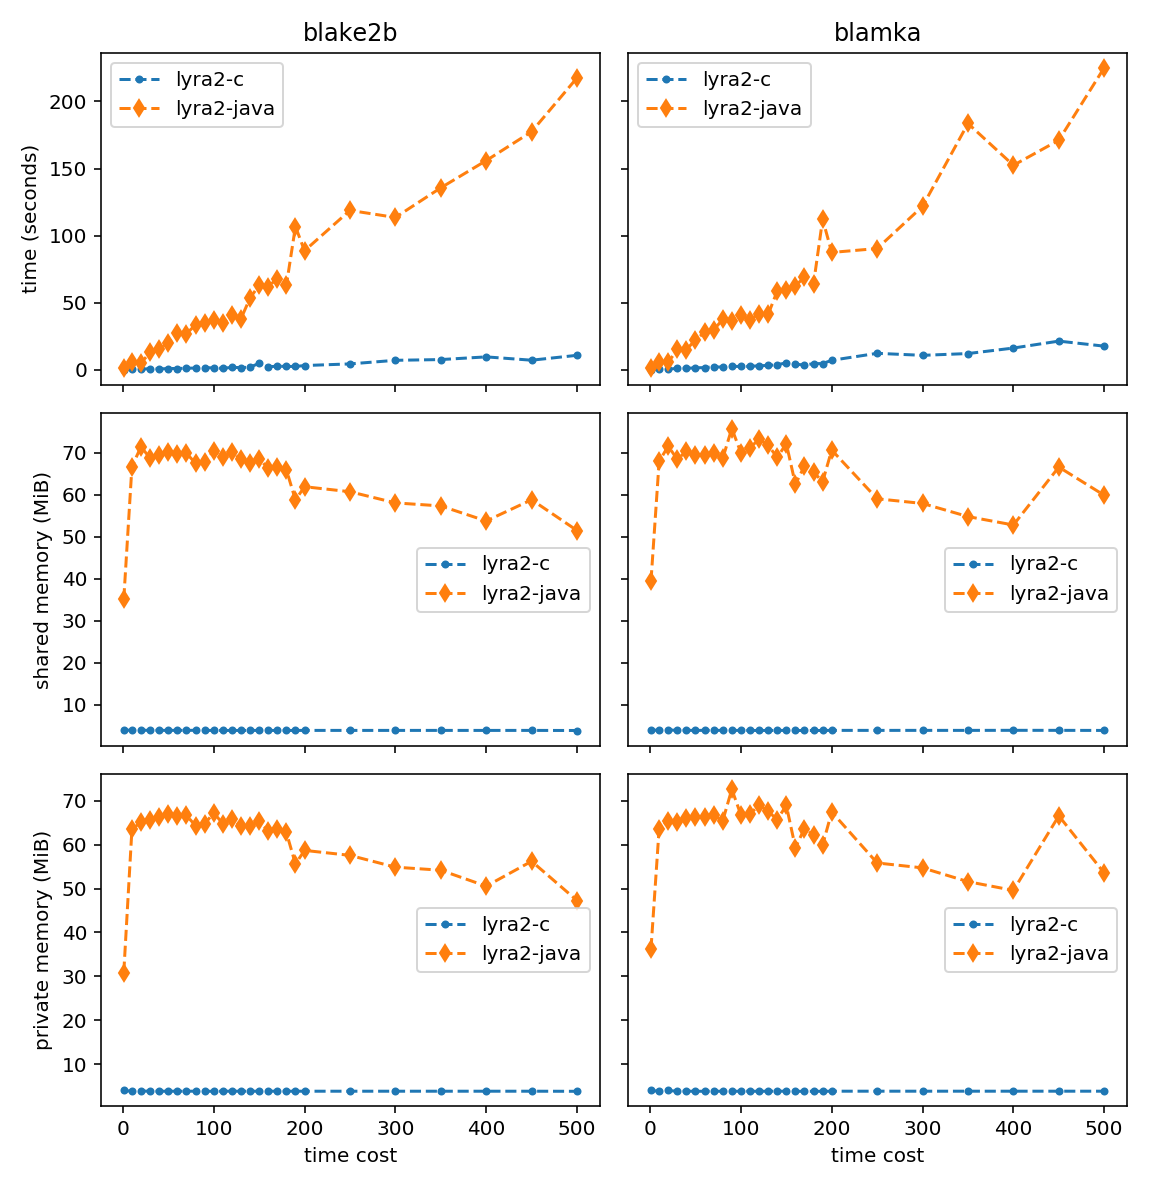
\includegraphics[width=\linewidth]{figures/tcost_2048}
    \caption{Original \texttt{lyra2-c} compared to \texttt{lyra2-java}: 2048 columns, fixed memory cost of 20}
    \label{figure:tcost_2048}
\end{figure}

\subsection{Changing time and memory costs}

There are four figures that show running time and memory consumption of Lyra2 when both time and memory costs change. Figures \ref{figure:tcost_mcost_blake2b_256} and \ref{figure:tcost_mcost_blake2b_2048} correspond to a 256- and 2048-column configurations of Lyra2 that both use the Blake2b sponge. Figures \ref{figure:tcost_mcost_blamka_256} and \ref{figure:tcost_mcost_blamka_2048} are the 256- and 2048-column configurations of Lyra2 with the BlaMka sponge. All of these four figures share the same properties. First of all, the original C implementation is still faster and consumes less memory than the Java one. Secondly, the running time as well as required space depend roughly linearly on the time and memory cost parameters simultaneously. The second observation goes somewhat against my intuition: my expectations where to see quadratic dependency since both the size of the matrix and the number of iterations are increased at the same time. 

\begin{figure}
    \centering
    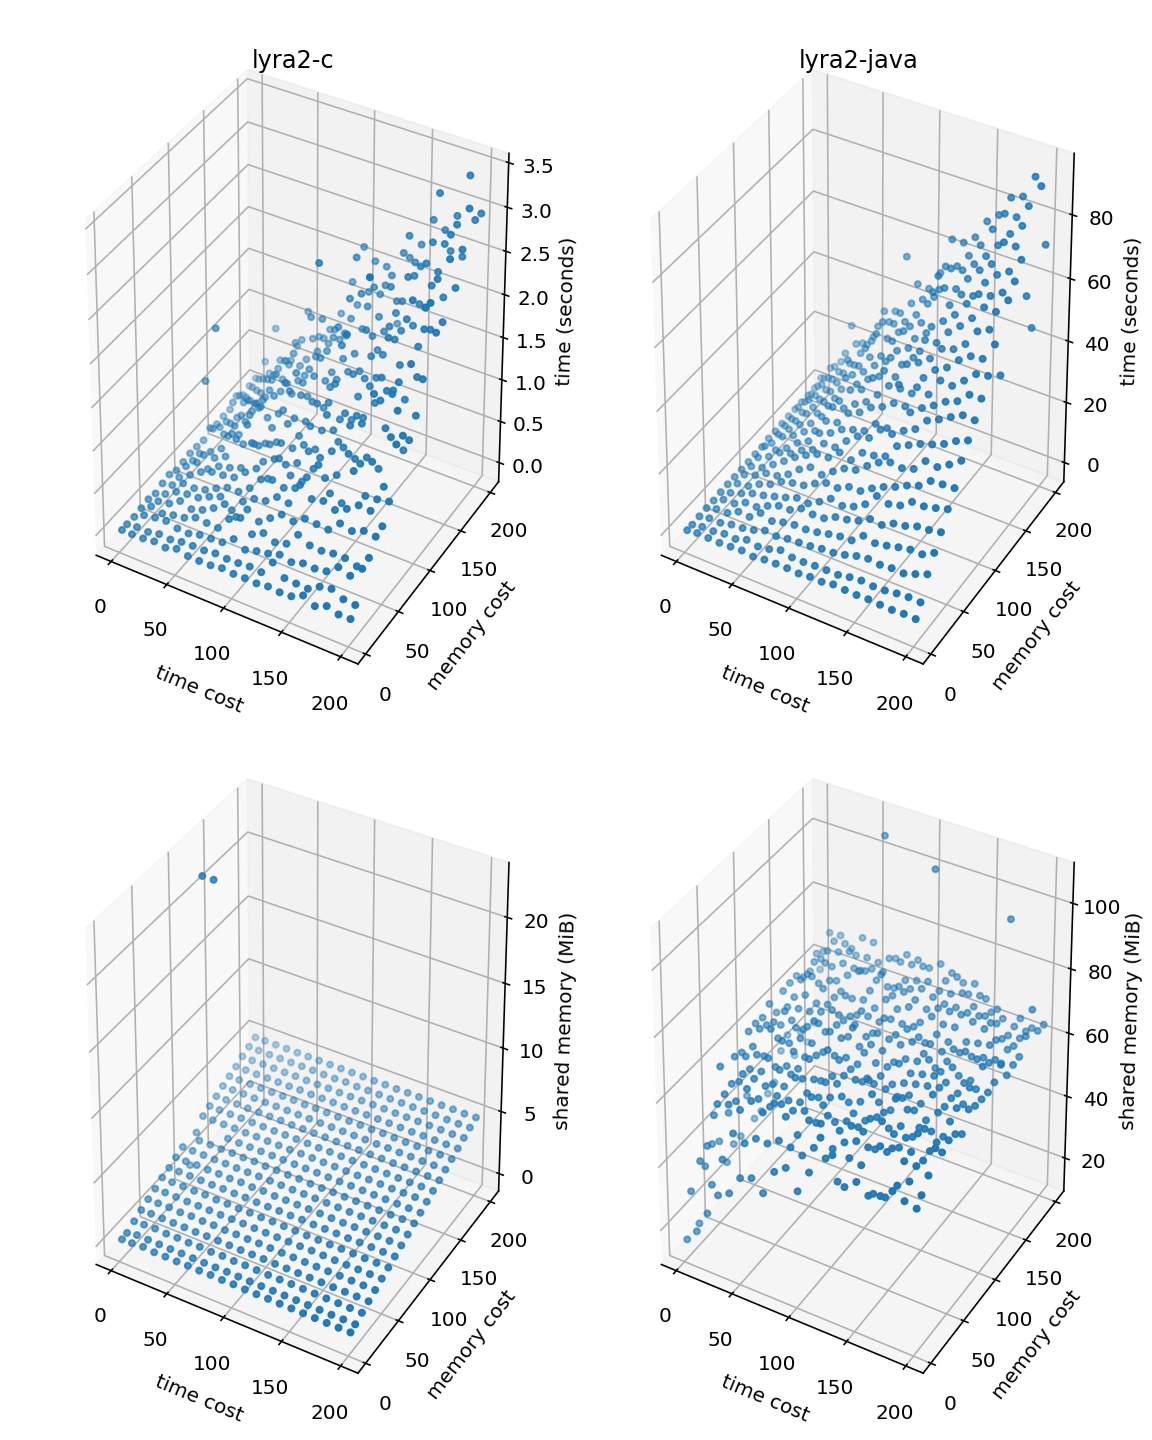
\includegraphics[width=\linewidth]{figures/tcost_mcost_blake2b_256}
    \caption{Original \texttt{lyra2-c} compared to \texttt{lyra2-java}: Blake2b sponge, 256 columns. TODO: java version still computing}
    \label{figure:tcost_mcost_blake2b_256}
\end{figure}

\begin{figure}
    \centering
    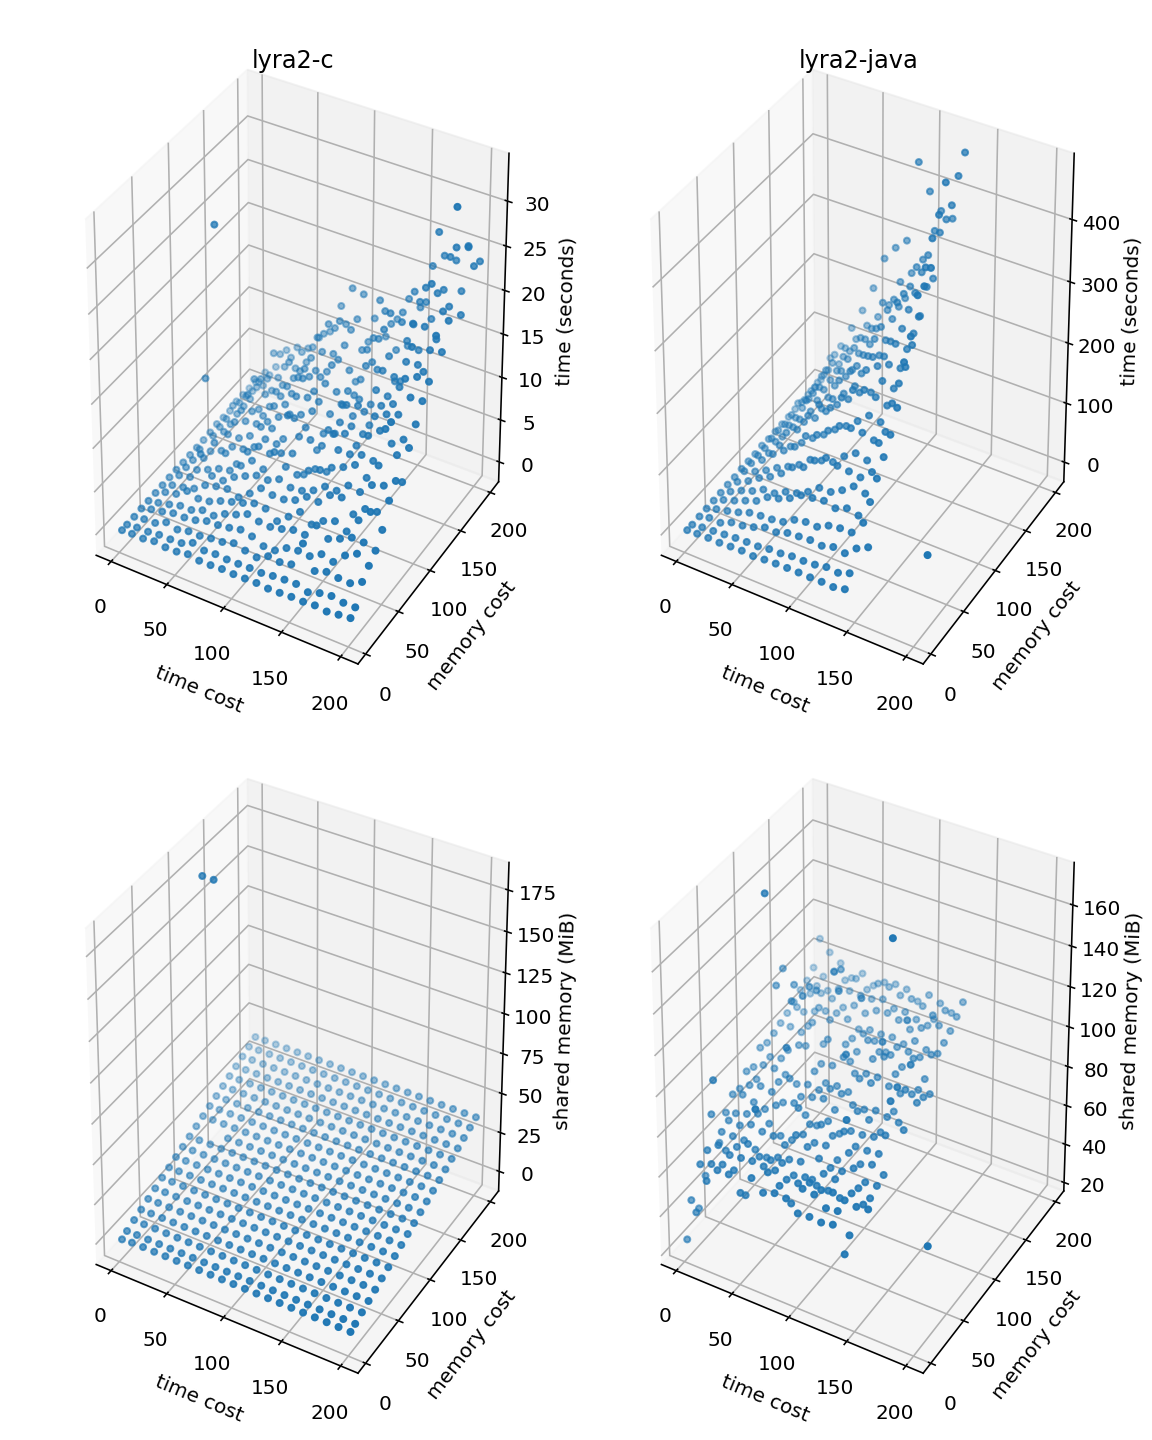
\includegraphics[width=\linewidth]{figures/tcost_mcost_blake2b_2048}
    \caption{Original \texttt{lyra2-c} compared to \texttt{lyra2-java}: Blake2b sponge, 2048 columns. TODO: java version still computing}
    \label{figure:tcost_mcost_blake2b_2048}
\end{figure}

\begin{figure}
    \centering
    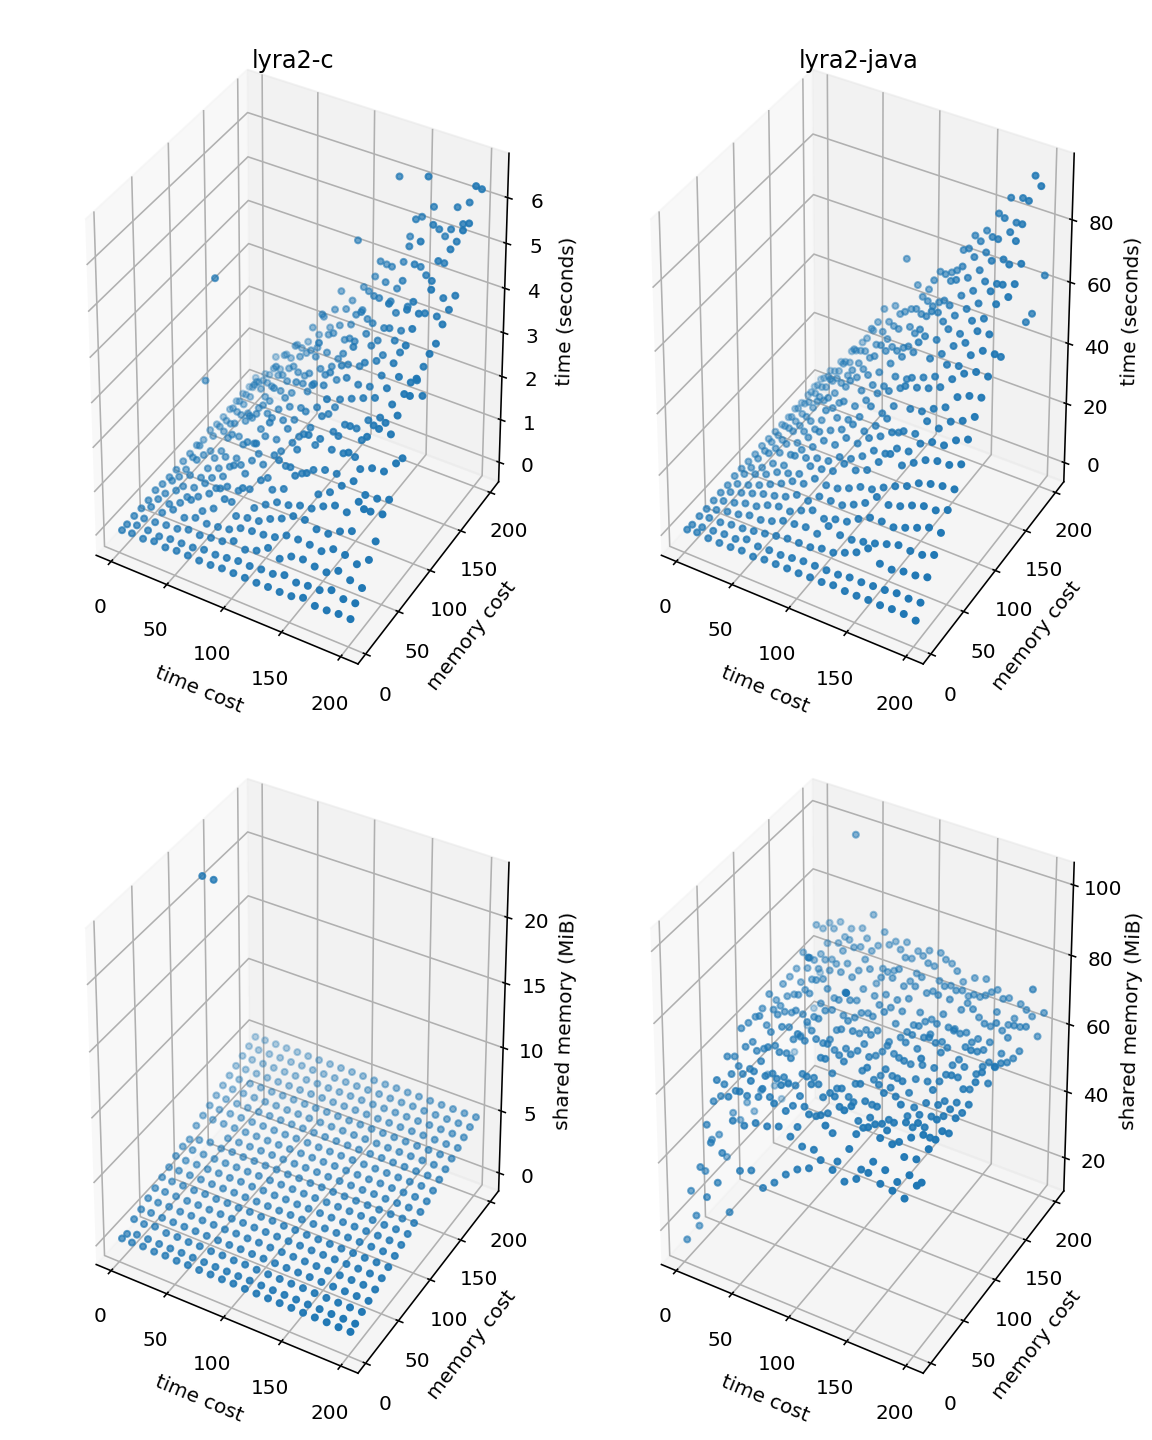
\includegraphics[width=\linewidth]{figures/tcost_mcost_blamka_256}
    \caption{Original \texttt{lyra2-c} compared to \texttt{lyra2-java}: BlaMka sponge, 256 columns. TODO: java version still computing}
    \label{figure:tcost_mcost_blamka_256}
\end{figure}

\begin{figure}
    \centering
    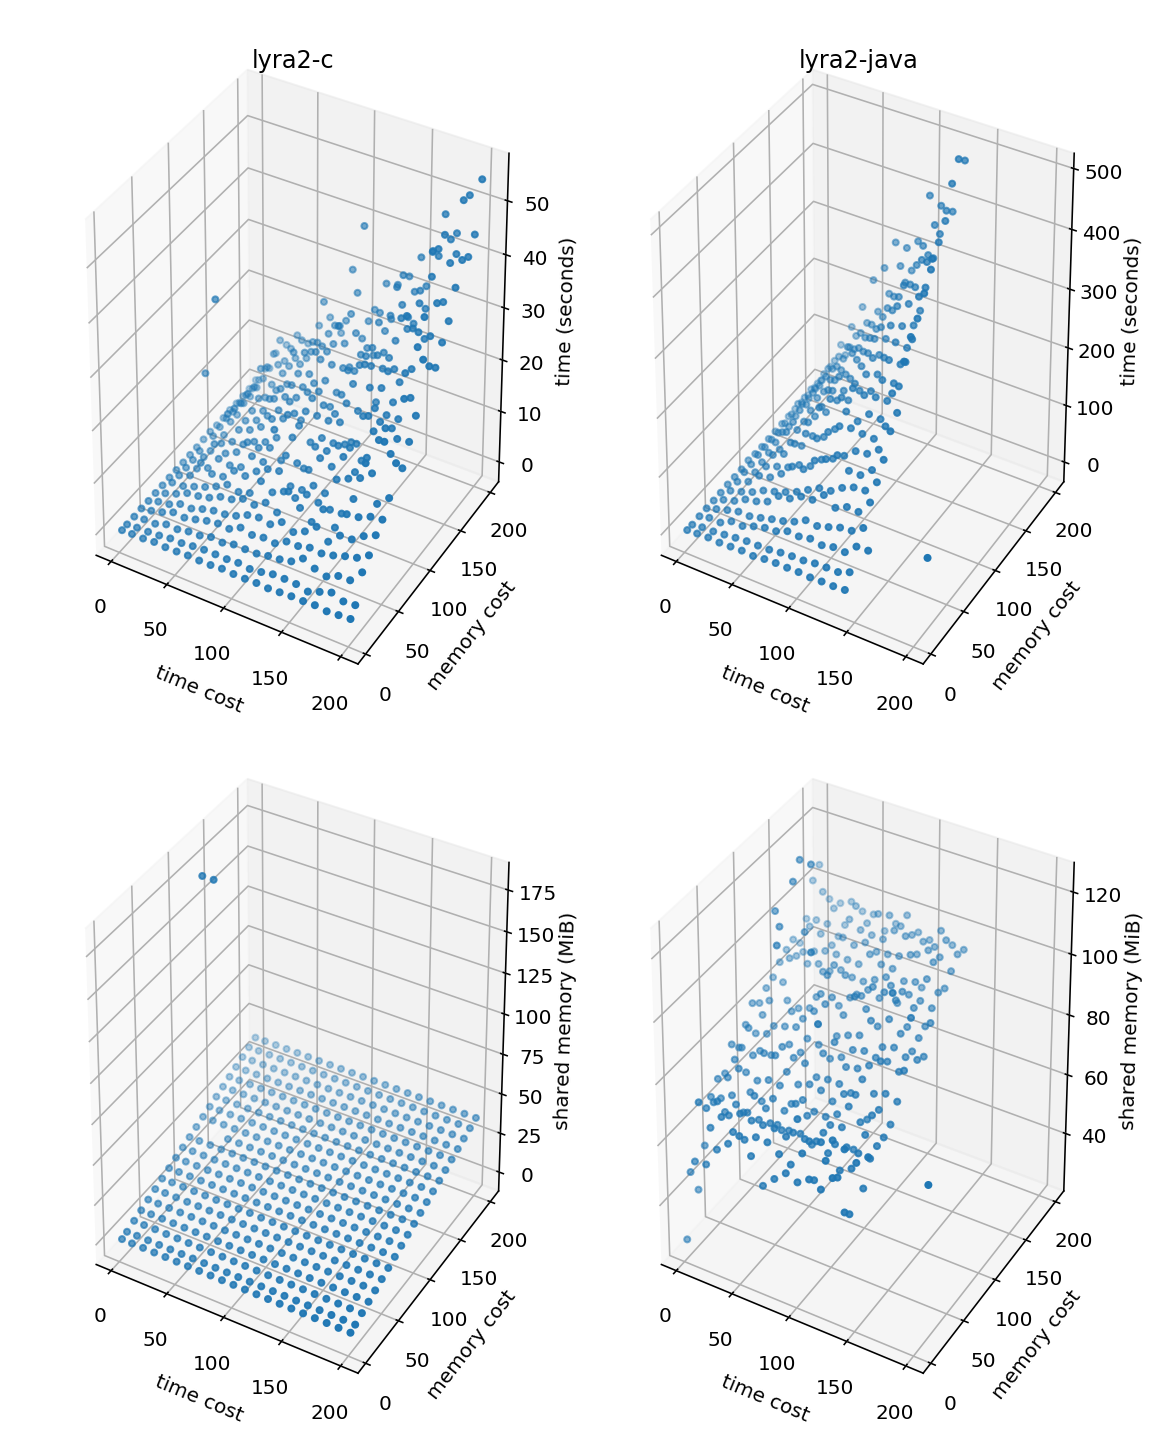
\includegraphics[width=\linewidth]{figures/tcost_mcost_blamka_2048}
    \caption{Original \texttt{lyra2-c} compared to \texttt{lyra2-java}: BlaMka sponge, 2048 columns. TODO: java version still computing}
    \label{figure:tcost_mcost_blamka_2048}
\end{figure}
